%%%%%%%%%%%%%%%%%%%%%%%%%%%%%%%%%%%%%%%%%%%%%%%%%%%%%
%%% Task 3 %%%%%%%%%%%%%%%%%%%%%%%%%%%%%%%%%%%%%%%%%%
%%%%%%%%%%%%%%%%%%%%%%%%%%%%%%%%%%%%%%%%%%%%%%%%%%%%%
\task{Induction machine}

%%%%%%%%%%%%%%%%%%%%%%%%%%%%%%%%%%%%%%%%%%%%%%
\taskGerman{Asynchronmaschine}


\subtask{Draw and label the stationary equivalent circuit diagram of the general induction machine. What simplification can you make if the machine is at standstill ($\omega_\mathrm{r}=\SI{0}{\per\second}$)?}{1}
\subtaskGerman{Zeichnen und beschriften Sie das stationäre Ersatzschaltbild der allgemeinen Asynchronmaschine. Welche Vereinfachung können Sie hierbei vornehmen, falls die Maschine stillsteht ($\omega_\mathrm{r}=\SI{0}{\per\second}$)?}

\begin{solutionblock}
    The general induction machine equivalent circuit diagram is given by:
    \begin{center}
        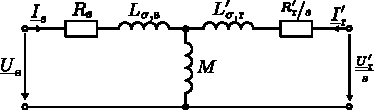
\includegraphics[width=0.6\textwidth]{../../lecture/fig/lec06/IM_T_ECD_steady_state.pdf}
    \end{center}
    If $\omega_\mathrm{r}=\SI{0}{\per\second}$ the mechanical rotor frequency is zero and the slip angular frequency is equal to the electrical angular frequency of the stator excitation: $\omega_\mathrm{s}= \omega_\mathrm{slip}$. Consequently, the slip ratio is equal to one ($s=\omega_\mathrm{slip}/\omega_\mathrm{s}=1$) and could be dropped from the equivalent circuit diagram.
\end{solutionblock}

\subtask{From now on consider a \textbf{squire cage induction machine} with the  parameters from Tab.~\ref{tab:characteristicsIM_task3}. Calculate the no-load speed $n_0$. }{2}
\subtaskGerman{Wir betrachten nun eine \textbf{Käfigläufer-Asynchronmaschine} mit den Parametern aus Tab.~\ref{tab:characteristicsIM_task3}. Berechnen Sie die Leerlaufdrehzahl $n_0$.}
\begin{table}[htb]
    \caption{Characteristics of the given induction machine.}
    \centering
    \begin{tabular}{lll}\toprule
    Symbol  & Description       & Values \\
    \midrule
    $U_{\mathrm{n}}$    & Nominal voltage           & $\SI{400}{\volt}$ \\
    $f_{\mathrm{s,n}}$  & Nominal frequency         & $\SI{60}{\hertz}$ \\
    $P_{\mathrm{n}}$    & Nominal power             & $\SI{20}{\kilo\watt}$ \\
    $n_{\mathrm{n}}$    & Nominal speed             & $\SI{1700}{\per\minute}$ \\
    $p$     & Pole pair number              & 2 \\
    \midrule
    $R_{\mathrm{s}}$    & Stator resistance         & $\SI{0}{\Omega}$ \\
    $R_{\mathrm{r}}'$    & Rotor resistance          & $\SI{2}{\ohm}$ \\
    $M$                 & Mutual inductance         & $\SI{70}{\milli\henry}$ \\
    $L_{\mathrm{\sigma,s}}$    & Stator leakage inductance  & $\SI{2}{\milli\henry}$ \\
    $L_{\mathrm{\sigma,r}}'$    & Rotor leakage inductance   & $\SI{2}{\milli\henry}$ \\
    \bottomrule
    \end{tabular}
    \label{tab:characteristicsIM_task3}
\end{table}

\begin{solutionblock}
    The no-load case is characterized by
    $$s = \frac{\omega_{\mathrm{slip}}}{\omega_{\mathrm{s}}} = \frac{0}{\omega_{\mathrm{s}}}=0, \qquad \omega_{\mathrm{s}} = \omega_{\mathrm{r,el}}.$$
    Hence, we have $$\omega_{\mathrm{s}} = 2\pi f_{\mathrm{s}} = 2\pi \cdot \SI{60}{\hertz} = \SI{377}{\per\second} = \omega_{\mathrm{r,el}}.$$ Converting this to the mechanical speed, we get
    $$n_0 = \frac{\omega_{\mathrm{r,el}}}{2 \pi p } \cdot \SI{60}{\second\per\minute} = \SI{1800}{\per\minute}.$$ 
\end{solutionblock}

\subtask{Calculate the nominal torque $T_\mathrm{n}$ and nominal slips $s_\mathrm{n}$.}{2}
\subtaskGerman{Berechnen Sie das Nennmoment $T_\mathrm{n}$ und den Nennschlupf $s_\mathrm{n}$.}

\begin{solutionblock}
    The nominal mechanical power is given by
    $$ P_{\mathrm{n}} = T_{\mathrm{n}} \omega_{\mathrm{r,n}}=T_{\mathrm{n}} 2\pi n_{\mathrm{n}} \SI{\frac{1}{60}}{\minute\per\second}.$$
    Hence, we can calculate the nominal torque as
    $$ T_{\mathrm{n}} = \frac{P_{\mathrm{n}} 60}{2\pi n_{\mathrm{n}}} \si{\second\per\minute}= \SI{112.35}{\newton\meter}.$$
    The slip angular frequency is 
    $$\omega_{\mathrm{slip,n}} = \omega_{\mathrm{s,n}} - \omega_{\mathrm{r,el,n}} = 2\pi (\SI{60}{\per\second} - \SI{\frac{2\cdot 1700}{60}}{\per\second}) = \SI{20.94}{\per\second}$$
    leading to a nominal slip of
    $$s_{\mathrm{n}} = \frac{\omega_{\mathrm{slip,n}}}{\omega_{\mathrm{s,n}}} = \frac{\SI{20.94}{\per\second}}{\SI{377}{\per\second}} = 0.0556.$$
\end{solutionblock}

\subtask{Determine the nominal electrical power $P_\mathrm{el,n}$ and the efficiency $\eta_\mathrm{n}$. For this purpose neglect the impact of the stator leakage inductance.}{2}
\subtaskGerman{Bestimmen Sie die Nennleistung $P_\mathrm{el,n}$ und den Wirkungsgrad $\eta_\mathrm{n}$. Vernachlässigen Sie hierbei den Einfluss der Statorstreuinduktivität.}

\begin{solutionblock}
    To determine the requested values, we first need to calculate the machine power losses. Since the stator ohmic losses can be neglected, we only have to consider the rotor ohmic losses. The nominal RMS rotor current is given by
    $$ I_{\mathrm{r,n}} = \frac{U_{\mathrm{n}}}{\sqrt{3}}\frac{1}{\sqrt{\frac{R_{\mathrm{r}}'}{s_\mathrm{n}}^2 + \left(\omega_{\mathrm{s}} L'_\mathrm{\sigma,r}\right)^2}} = \SI{230.94}{\volt} \cdot\frac{1}{\sqrt{(\SI{35.71}{\ohm})^2 + (\SI{0.75}{\ohm})^2}} = \SI{230.94}{\volt} \cdot \frac{1}{\SI{35.72}{\ohm}} = \SI{6.47}{\ampere}. $$
    The power losses of the rotor are then 
    $$ P_{\mathrm{r,l,n}} = \frac{3}{2} (I_{\mathrm{r,n}})^2 \frac{R_{\mathrm{r}}'}{s_\mathrm{n}} = \frac{3}{2} \cdot \SI{31.80}{\ampere\squared} \cdot \SI{35.72}{\ohm} = \SI{1492.91}{\watt}.$$
    The total electrical power sums up to
    $$ P_{\mathrm{el,n}} = P_{\mathrm{n}} + P_{\mathrm{r,l,n}} = \SI{20}{\kilo\watt} + \SI{1.49}{\kilo\watt} = \SI{21.49}{\kilo\watt}.$$
    The efficiency is then
    $$ \eta_{\mathrm{n}} = \frac{P_{\mathrm{n}}}{P_{\mathrm{el,n}}} = \frac{\SI{20}{\kilo\watt}}{\SI{21.49}{\kilo\watt}} = 0.931 = \SI{93.1}{\percent}.$$
\end{solutionblock}

\subtask{Determine the maximum possible torque $T_\mathrm{max}$ of the machine. Which speed $n_\mathrm{max}$ corresponds to that operating point?}{2}
\subtaskGerman{Bestimmen Sie das maximale Drehmoment $T_\mathrm{max}$ der Maschine. Welche Drehzahl $n_\mathrm{max}$ entspricht dieser Betriebspunkt?}

\begin{solutionblock}
    The maximum achievable torque is 
    $$ T_\mathrm{max} = \frac{3}{2} p \frac{U_\mathrm{s}^2}{\omega_\mathrm{s}^2}\frac{M^2}{\sigma (L_{\sigma,\mathrm{s}} +M)^2(L'_{\sigma,\mathrm{r}} +M)} = \frac{3}{2} \cdot2 \cdot \frac{(\SI{230.94}{\volt})^2}{(\SI{376.99}{\per\second})^2} \cdot\frac{(\SI{70}{\milli\henry})^2}{0.055\cdot(\SI{72}{\milli\henry})^3} = \SI{268.72}{\newton\metre}.$$
    The corresponding slip frequency is
    $$ \omega_{\mathrm{max}} = \frac{R'_\mathrm{r}}{\sigma (L'_{\sigma,\mathrm{r}} +M)} = \frac{\SI{2}{\ohm}}{0.055\cdot(\SI{72}{\milli\henry})} = \SI{416.6}{\per\second}$$
    leading to a rotor angular speed of
    $$ \omega_{\mathrm{r,max}} = \frac{1}{p} (\omega_\mathrm{s} - \omega_{\mathrm{max}}) = \SI{-19.81}{\per\second}$$
    resulting in a mechanical speed of
    $$ n_{\mathrm{max}} = \frac{\omega_{r,\mathrm{max}}}{2\pi} \cdot \SI{60}{\second\per\minute} = \SI{-2.07}{\per\minute}.$$
    Hence, the maximum torque is achieved at a negative speed which is necessary due to the relatively large slip frequency at the maximum torque operating point (which is mostly due to the relatively large rotor resistance).
\end{solutionblock}
